\documentclass[12pt, a4paper]{report}

% ─── Packages ─────────────────────────────────────────────────────────────────
\usepackage[T1]{fontenc}
\usepackage[utf8]{inputenc}
\usepackage{palatino}
\usepackage[margin=2.5cm]{geometry}
\usepackage{graphicx}
\usepackage{booktabs}
\usepackage{amsmath, amssymb, bm}
\usepackage{hyperref}
\usepackage{float}
\usepackage{caption}
\usepackage{subcaption}
\usepackage{parskip}
\usepackage{microtype}
\usepackage{xcolor}
\usepackage{titlesec}
\usepackage{fancyhdr}
\usepackage{enumitem}

% ─── Section formatting ───────────────────────────────────────────────────────
\titleformat{\chapter}[hang]{\LARGE\bfseries}{\thechapter}{1em}{}
\titlespacing{\chapter}{0pt}{0pt}{20pt}

% ─── Hyperref ─────────────────────────────────────────────────────────────────
\hypersetup{
    colorlinks=true,
    linkcolor=black,
    citecolor=black,
    urlcolor=blue,
}

% ─── Header/Footer ────────────────────────────────────────────────────────────
\pagestyle{fancy}
\fancyhf{}
\fancyhead[L]{\small Deep Learning -- Lab 6: Conditional Generative Models on iCLEVR}
\fancyhead[R]{\small\thepage}
\renewcommand{\headrulewidth}{0.4pt}

% ─── Title info ───────────────────────────────────────────────────────────────
\title{}
\date{}

% ══════════════════════════════════════════════════════════════════════════════
\begin{document}

% ─── Title Page ───────────────────────────────────────────────────────────────
\begin{titlepage}
\centering
\vspace*{3cm}
{\LARGE\bfseries Deep Learning\par}
\vspace{0.5em}
{\Large Lab 6\par}
\vspace{0.5em}
{\large Conditional Generative Models on iCLEVR\par}

\vspace{1cm}
\rule{0.6\linewidth}{0.8pt}

\vspace{2cm}
{\large\textbf{Student ID}\\[0.3em] B11107122\par}

\vspace{1em}
{\large\textbf{Name}\\[0.3em] Yue-Lin Tu\par}

\vspace{1em}
{\large\textbf{School}\\[0.3em] National Taiwan University of Science and Technology\par}

\vfill
\rule{0.6\linewidth}{0.8pt}\\[0.5em]
{\small Due Date: 2026/05/12}
\end{titlepage}

% ─── Table of Contents ────────────────────────────────────────────────────────
\tableofcontents
\clearpage

% ══════════════════════════════════════════════════════════════════════════════
\chapter{Introduction}

\section*{Lab Objectives \& Overview}

This report presents a Conditional Denoising Diffusion Probabilistic Model (DDPM)
trained on the iCLEVR dataset to generate $64\times64$ RGB images of 3D objects
conditioned on a 24-dimensional multi-label binary vector.
Given a set of object labels (e.g.\ ``red sphere'', ``cyan cylinder'', ``cyan cube''),
the model synthesises scenes containing exactly those objects.
Generated images are evaluated by a pretrained ResNet18 classifier that returns a
multi-label accuracy score.

\section*{Key Findings}

The model achieves \textbf{95.83\%} accuracy on \texttt{test.json} and
\textbf{98.81\%} on \texttt{new\_test.json} (DDIM, 100 steps, classifier guidance
scale $s=2.0$, EMA weights), both well above the 80\% full-credit threshold.
An ablation study over sampling strategies, DDIM step counts, and guidance scales
confirms that moderate guidance ($s\approx2$) and at least 100 DDIM steps
provide the best quality--speed trade-off.

\section*{Report Organization}

Chapter~2 covers the complete implementation: dataset pipeline, cosine noise
schedule, Conditional UNet architecture, conditioning mechanism, training procedure,
and all three sampling strategies with full mathematical derivations.
Chapter~3 presents the generated image grids, denoising visualisation, and accuracy
results including terminal output screenshots.
Chapter~4 contains the ablation study comparing samplers, step counts, guidance
scales, and EMA versus raw weights.

% ══════════════════════════════════════════════════════════════════════════════
\chapter{Implementation Details}

\section{Dataset and Preprocessing}

The iCLEVR dataset contains 18{,}009 training images.
Each image is paired with a list of object label strings from a vocabulary of 24
categories encoded in \texttt{objects.json}.

\textbf{Multi-label one-hot encoding.}
For a sample whose label list is $\mathcal{L}$, the condition vector is
\[
  \mathbf{c} \in \{0,1\}^{24},\qquad c_k = \mathbf{1}[k \in \mathcal{L}].
\]

\textbf{Image normalisation.}
Raw pixel values $p \in [0,255]$ are normalised to $[-1,1]$:
\[
  \tilde{x} = 2\,\frac{p}{255} - 1,
\]
matching \texttt{Normalize((0.5, 0.5, 0.5),(0.5, 0.5, 0.5))}.
The pretrained evaluator requires this normalisation; denormalization $x \mapsto (x+1)/2$
is applied before saving output images.

\section{Cosine Noise Schedule}

A cosine variance schedule~\cite{nichol2021improved} is used over $T=1{,}000$ timesteps.
Define the auxiliary function
\[
  f(t) = \cos^2\!\left(\frac{t/T + s_0}{1 + s_0} \cdot \frac{\pi}{2}\right),
  \qquad s_0 = 0.008,
\]
from which the cumulative noise level and step-wise variance are derived:
\[
  \bar{\alpha}_t = \frac{f(t)}{f(0)},
  \qquad
  \beta_t = \min\!\left(1 - \frac{\bar{\alpha}_t}{\bar{\alpha}_{t-1}},\; 0.999\right),
  \qquad
  \alpha_t = 1 - \beta_t.
\]
The cosine schedule ensures $\bar{\alpha}_t$ decays smoothly and avoids the abrupt
transition to near-zero signal that the linear schedule produces at large $t$, leading
to better image quality at inference.

\section{Forward Diffusion Process}

The forward process is a fixed Markov chain:
\[
  q(\mathbf{x}_t \mid \mathbf{x}_{t-1})
    = \mathcal{N}\!\bigl(\mathbf{x}_t;\;
        \sqrt{1-\beta_t}\,\mathbf{x}_{t-1},\; \beta_t\mathbf{I}\bigr).
\]
Telescoping the Markov chain yields a closed-form expression for the
noisy sample at any timestep $t$ (reparameterisation):
\[
  \mathbf{x}_t
    = \sqrt{\bar\alpha_t}\,\mathbf{x}_0
    + \sqrt{1-\bar\alpha_t}\,\boldsymbol\epsilon,
  \qquad
  \boldsymbol\epsilon \sim \mathcal{N}(\mathbf{0},\mathbf{I}).
\]
This allows the model to sample $\mathbf{x}_t$ directly from $\mathbf{x}_0$ in one step
during training, without any loop.

\section{Training Objective}

The reverse process models
$p_\theta(\mathbf{x}_{t-1}\mid\mathbf{x}_t, \mathbf{c})
  = \mathcal{N}(\bm\mu_\theta, \tilde\beta_t\mathbf{I})$,
with posterior variance
$\tilde\beta_t = \frac{1-\bar\alpha_{t-1}}{1-\bar\alpha_t}\beta_t$.
The optimal posterior mean is
\[
  \tilde{\bm\mu}_t
    = \frac{\sqrt{\bar\alpha_{t-1}}\,\beta_t}{1-\bar\alpha_t}\,\mathbf{x}_0
    + \frac{\sqrt{\alpha_t}(1-\bar\alpha_{t-1})}{1-\bar\alpha_t}\,\mathbf{x}_t.
\]
Parameterising by the noise $\boldsymbol\epsilon_\theta$ gives
\[
  \bm\mu_\theta(\mathbf{x}_t,t,\mathbf{c})
    = \frac{1}{\sqrt{\alpha_t}}\!\left(
        \mathbf{x}_t
        - \frac{\beta_t}{\sqrt{1-\bar\alpha_t}}
          \boldsymbol\epsilon_\theta(\mathbf{x}_t,t,\mathbf{c})
      \right).
\]
Ho et al.~\cite{ho2020ddpm} show this leads to the simplified objective:
\[
  \mathcal{L}_{\text{simple}}
    = \mathbb{E}_{t,\mathbf{x}_0,\boldsymbol\epsilon}\!\left[
        \left\|\boldsymbol\epsilon
          - \boldsymbol\epsilon_\theta\!\left(
              \sqrt{\bar\alpha_t}\,\mathbf{x}_0
              + \sqrt{1-\bar\alpha_t}\,\boldsymbol\epsilon,\;
              t,\; \mathbf{c}
            \right)\right\|^2
      \right].
\]
In practice: for each training step, uniformly sample $t \sim \mathcal{U}\{0,\ldots,T{-}1\}$,
sample noise $\boldsymbol\epsilon \sim \mathcal{N}(\mathbf{0},\mathbf{I})$, compute
$\mathbf{x}_t$, predict $\hat{\boldsymbol\epsilon}$, and minimise the MSE.

\section{Conditional UNet Architecture}

\subsection{Time Embedding}

A sinusoidal positional encoding maps scalar timestep $t$ to a $d_t = 128$ vector:
\[
  \mathrm{TE}(t)_{2i}   = \sin\!\left(\frac{t}{10{,}000^{2i/d_t}}\right),\quad
  \mathrm{TE}(t)_{2i+1} = \cos\!\left(\frac{t}{10{,}000^{2i/d_t}}\right),\quad
  i = 0,\ldots,\tfrac{d_t}{2}-1.
\]
This is then expanded to a 512-dimensional latent via an MLP:
\[
  \mathbf{t}_e
    = \mathrm{Linear}_{512\to512}\!\Bigl(
        \mathrm{SiLU}\bigl(
          \mathrm{Linear}_{128\to512}(\mathrm{TE}(t))
        \bigr)
      \Bigr) \in \mathbb{R}^{512}.
\]

\subsection{Label Embedding}

The 24-dimensional condition $\mathbf{c}$ is projected through an MLP:
\[
  \mathbf{c}_e
    = \mathrm{Linear}_{256\to256}\!\Bigl(
        \mathrm{SiLU}\bigl(
          \mathrm{Linear}_{24\to256}(\mathbf{c})
        \bigr)
      \Bigr) \in \mathbb{R}^{256}.
\]
The combined condition is $\mathbf{e} = [\mathbf{t}_e \;\|\; \mathbf{c}_e] \in \mathbb{R}^{768}$.

\subsection{Adaptive Group Normalisation (AdaGN)}

Following~\cite{dhariwal2021beatgans}, each ResBlock injects the condition via AdaGN.
Given a feature map $\mathbf{h} \in \mathbb{R}^{C \times H \times W}$, a linear
projection of the condition yields channel-wise scale and shift parameters:
\[
  (\boldsymbol\gamma,\, \boldsymbol\delta)
    = \mathrm{Linear}_{768 \to 2C}(\mathbf{e})
    \in \mathbb{R}^{C} \times \mathbb{R}^{C}.
\]
The normalised feature map is then modulated as:
\[
  \mathbf{h}
    \leftarrow \mathrm{GN}_{32}(\mathbf{h}) \odot (1 + \boldsymbol\gamma)
               + \boldsymbol\delta,
\]
where $\mathrm{GN}_{32}$ is Group Normalization with 32 groups and $\odot$ denotes
channel-wise multiplication.
Every layer thus adapts its feature statistics independently to both the timestep
and the class condition.
The last convolution in each ResBlock is zero-initialised so the block starts as an
approximate identity mapping, stabilising early training.

\subsection{Multi-Head Self-Attention}

Self-attention is applied after every ResBlock at spatial resolutions $32\times32$,
$16\times16$, and $8\times8$.
The number of heads is $n_h = \max(1, \lfloor C/64 \rfloor)$ with 64 channels per head.
Given flattened spatial tokens $\mathbf{Q},\mathbf{K},\mathbf{V} \in \mathbb{R}^{HW \times d_k}$:
\[
  \mathrm{Attn}(\mathbf{Q},\mathbf{K},\mathbf{V})
    = \mathrm{softmax}\!\left(\frac{\mathbf{Q}\mathbf{K}^\top}{\sqrt{d_k}}\right)\mathbf{V}.
\]

\subsection{Encoder--Decoder Structure}

\begin{table}[H]
\centering
\caption{UNet channel configuration. Ch.\ mult.\ $= (1, 2, 2, 4)$, base $= 128$.}
\begin{tabular}{llcl}
\toprule
Stage & Resolution & Channels & Components \\
\midrule
Input conv   & $64\times64$ & $128$ & $3\to128$ conv \\
Encoder L1   & $64\to32$    & $128$ & 2$\times$(ResBlock), Downsample \\
Encoder L2   & $32\to16$    & $256$ & 2$\times$(ResBlock + Attn), Downsample \\
Encoder L3   & $16\to8$     & $256$ & 2$\times$(ResBlock + Attn), Downsample \\
Encoder L4   & $8\times8$   & $512$ & 2$\times$(ResBlock + Attn) \\
Bottleneck   & $8\times8$   & $512$ & ResBlock + Attn + ResBlock \\
Decoder L4   & $8\to16$     & $512$ & 2$\times$(ResBlock + Attn), Upsample \\
Decoder L3   & $16\to32$    & $256$ & 2$\times$(ResBlock + Attn), Upsample \\
Decoder L2   & $32\to64$    & $256$ & 2$\times$(ResBlock + Attn), Upsample \\
Decoder L1   & $64\times64$ & $128$ & 2$\times$(ResBlock) \\
Output conv  & $64\times64$ & $3$   & $128\to3$ conv (zero-init) \\
\bottomrule
\end{tabular}
\end{table}

Skip connections concatenate encoder outputs with decoder inputs (channel doubling before
each decoder ResBlock).
Downsampling uses a strided convolution (stride 2); upsampling uses nearest-neighbour
interpolation followed by a convolution (BigGAN-style).

\section{Training Configuration}

\begin{table}[H]
\centering
\caption{Training hyperparameters.}
\begin{tabular}{ll}
\toprule
Hyperparameter & Value \\
\midrule
Optimiser                & AdamW, $\beta_1{=}0.9$, $\beta_2{=}0.999$ \\
Learning rate            & $2\times10^{-4}$ \\
Weight decay             & $10^{-4}$ \\
LR schedule              & CosineAnnealingLR, $T_{\max}=200$ epochs \\
Batch size               & 64 \\
Precision                & Mixed (AMP) \\
Gradient clipping        & $\|\nabla\|_2 \le 1.0$ \\
EMA decay $\lambda$      & 0.9999, warmup after 2{,}000 steps \\
Training epochs          & 200 ($\approx617$ min on single GPU) \\
Final training loss      & $\approx 0.0012$ \\
\bottomrule
\end{tabular}
\end{table}

\textbf{Exponential Moving Average (EMA).}
Shadow weights $\hat\theta$ track the trainable parameters $\theta$:
\[
  \hat\theta \;\leftarrow\; \lambda\,\hat\theta + (1-\lambda)\,\theta,
  \qquad \lambda = 0.9999.
\]
EMA weights are used exclusively at inference; they smooth out high-frequency
parameter oscillations and consistently produce sharper, more coherent images.

\section{Sampling Methods}

\subsection{DDPM Sampling}

Standard ancestral sampling~\cite{ho2020ddpm} runs all $T=1{,}000$ steps:
\[
  \mathbf{x}_{t-1}
    = \underbrace{
        \frac{1}{\sqrt{\alpha_t}}\!\left(
          \mathbf{x}_t
          - \frac{\beta_t}{\sqrt{1-\bar\alpha_t}}
            \boldsymbol\epsilon_\theta(\mathbf{x}_t, t, \mathbf{c})
        \right)
      }_{\text{predicted mean}}
    + \underbrace{\sqrt{\tilde\beta_t}\,\mathbf{z}}_{\text{noise}},
  \qquad \mathbf{z} \sim \mathcal{N}(\mathbf{0},\mathbf{I}).
\]

\subsection{DDIM Sampling}

DDIM~\cite{song2020ddim} derives a deterministic ($\eta=0$) sub-sequence sampler
that skips timesteps, enabling generation in $S \ll T$ steps.
First, the predicted clean image is recovered:
\[
  \hat{\mathbf{x}}_0
    = \frac{
        \mathbf{x}_t
        - \sqrt{1-\bar\alpha_t}\;
          \boldsymbol\epsilon_\theta(\mathbf{x}_t, t, \mathbf{c})
      }{\sqrt{\bar\alpha_t}}.
\]
The deterministic update step then interpolates between the predicted clean image and
the predicted noise direction:
\[
  \mathbf{x}_{t'}
    = \sqrt{\bar\alpha_{t'}}\;\hat{\mathbf{x}}_0
    + \sqrt{1-\bar\alpha_{t'}}\;
      \boldsymbol\epsilon_\theta(\mathbf{x}_t, t, \mathbf{c}),
\]
where $t'$ is the previous timestep in the chosen sub-sequence.
At $S=100$ steps this is $10\times$ faster than DDPM at 1{,}000 steps.

\subsection{DDIM with Classifier Guidance}

Following~\cite{dhariwal2021beatgans}, the provided frozen ResNet18 evaluator
$f_\phi$ acts as a classifier whose gradient steers generation.
Guidance is applied in the predicted $\hat{\mathbf{x}}_0$ space:

\begin{enumerate}[noitemsep]
  \item Predict the clean image:
    $\hat{\mathbf{x}}_0
      = \bigl(\mathbf{x}_t
        - \sqrt{1-\bar\alpha_t}\;
          \boldsymbol\epsilon_\theta(\mathbf{x}_t,t,\mathbf{c})\bigr)
      / \sqrt{\bar\alpha_t}$.

  \item Compute the BCE guidance gradient with respect to $\hat{\mathbf{x}}_0$:
    \[
      \mathbf{g}
        = \nabla_{\hat{\mathbf{x}}_0}\,
          \mathcal{L}_{\mathrm{BCE}}\!\bigl(
            f_\phi(\hat{\mathbf{x}}_0),\; \mathbf{c}
          \bigr).
    \]

  \item Apply guidance and clamp for stability:
    \[
      \hat{\mathbf{x}}_0^*
        = \mathrm{clamp}\!\left(
            \hat{\mathbf{x}}_0 - s\cdot\mathbf{g},\; -1,\; 1
          \right).
    \]

  \item Re-derive the guided noise estimate:
    \[
      \hat{\boldsymbol\epsilon}^*
        = \frac{
            \mathbf{x}_t
            - \sqrt{\bar\alpha_t}\;\hat{\mathbf{x}}_0^*
          }{\sqrt{1-\bar\alpha_t}}.
    \]

  \item Take the DDIM step with $\hat{\boldsymbol\epsilon}^*$:
    \[
      \mathbf{x}_{t'}
        = \sqrt{\bar\alpha_{t'}}\;\hat{\mathbf{x}}_0^*
        + \sqrt{1-\bar\alpha_{t'}}\;\hat{\boldsymbol\epsilon}^*.
    \]
\end{enumerate}

The guidance scale $s$ controls the condition-adherence strength.
The ablation (Chapter~4) shows $s=2.0$ is optimal.

% ══════════════════════════════════════════════════════════════════════════════
\chapter{Results}

\section{Generated Images}

Figures~\ref{fig:test_grid} and~\ref{fig:newtest_grid} show the $8\times4$
grids of 32 generated images for \texttt{test.json} and \texttt{new\_test.json}
using the best configuration (DDIM, 100 steps, guidance $s=2.0$, EMA weights).

\begin{figure}[H]
  \centering
  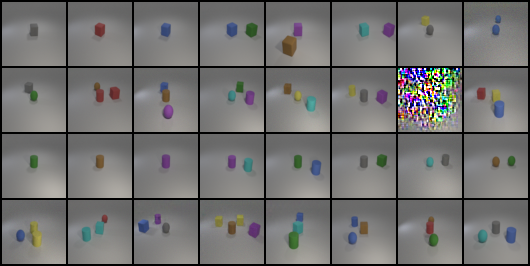
\includegraphics[width=0.92\linewidth]{../DL_LAB6_B11107122_凃岳霖/results/test_guided_s2_grid.png}
  \caption{Synthetic images for \texttt{test.json} (DDIM 100 steps, guidance $s=2.0$).}
  \label{fig:test_grid}
\end{figure}

\begin{figure}[H]
  \centering
  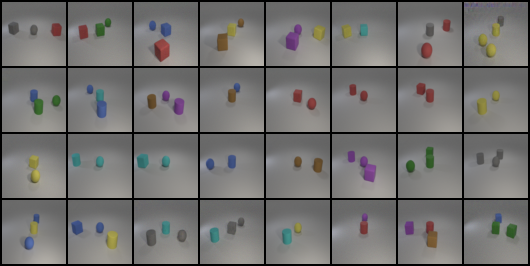
\includegraphics[width=0.92\linewidth]{../DL_LAB6_B11107122_凃岳霖/results/new_test_guided_s2_grid.png}
  \caption{Synthetic images for \texttt{new\_test.json} (DDIM 100 steps, guidance $s=2.0$).}
  \label{fig:newtest_grid}
\end{figure}

\section{Denoising Process}

Figure~\ref{fig:denoise} visualises 8 evenly-spaced snapshots of the reverse diffusion
chain for the fixed condition \texttt{["red sphere", "cyan cylinder", "cyan cube"]},
using the DDPM sampler.

\begin{figure}[H]
  \centering
  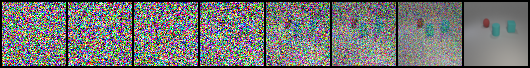
\includegraphics[width=\linewidth]{../DL_LAB6_B11107122_凃岳霖/results/denoise_process.png}
  \caption{Denoising process: from pure Gaussian noise $\mathbf{x}_T$ (left) to the
           generated image $\mathbf{x}_0$ (right). DDPM sampler, 1{,}000 steps.
           Condition: red sphere + cyan cylinder + cyan cube.}
  \label{fig:denoise}
\end{figure}

\section{Accuracy}

Figure~\ref{fig:acc_screenshot} shows the terminal output of the evaluator for the
best configuration.
Both scores exceed $0.8$, placing the model in the 100\% grade tier.

\begin{figure}[H]
  \centering
  \fbox{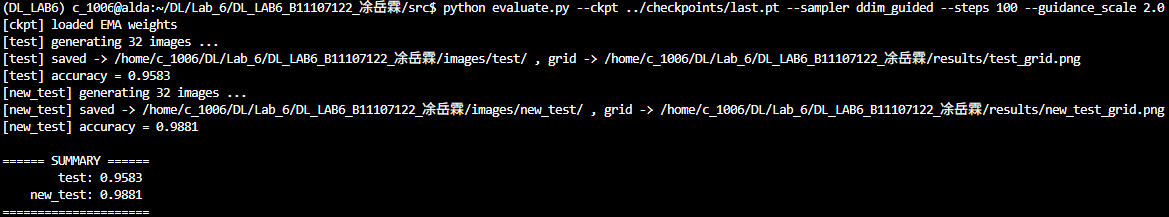
\includegraphics[width=0.92\linewidth]{figures/accuracy_screenshot.png}}
  \caption{Evaluator terminal output: \texttt{test} accuracy $= 0.9583$,
           \texttt{new\_test} accuracy $= 0.9881$
           (DDIM, 100 steps, guidance scale $s=2.0$, EMA weights).}
  \label{fig:acc_screenshot}
\end{figure}

\begin{table}[H]
\centering
\caption{Accuracy summary across configurations. All entries use EMA weights,
         200-epoch checkpoint.}
\begin{tabular}{lcc}
\toprule
Configuration & \texttt{test} & \texttt{new\_test} \\
\midrule
DDIM, 100 steps, $s=2.0$ (\textbf{best}) & \textbf{0.9583} & \textbf{0.9881} \\
DDIM, 100 steps, $s=3.0$                 & 0.9444 & 0.9167 \\
DDPM, 1{,}000 steps                      & 0.9722 & 0.9286 \\
No EMA (raw weights)                     & 0.9444 & 0.9167 \\
\bottomrule
\end{tabular}
\end{table}

% ══════════════════════════════════════════════════════════════════════════════
\chapter{Ablation Studies}

\section{Sampler and Number of Steps}

\begin{table}[H]
\centering
\caption{Sampler ablation (EMA weights, no classifier guidance).}
\begin{tabular}{lccc}
\toprule
Sampler & Steps & \texttt{test} & \texttt{new\_test} \\
\midrule
DDPM & 100   & 0.9583 & 0.9286 \\
DDPM & 1{,}000 & 0.9722 & 0.9286 \\
DDIM & 25    & 0.9444 & 0.9048 \\
DDIM & 50    & 0.9167 & 0.9167 \\
DDIM & 100   & 0.9444 & 0.9167 \\
DDIM & 200   & 0.9722 & 0.9048 \\
\bottomrule
\end{tabular}
\end{table}

DDPM with 1{,}000 steps achieves the best test accuracy (0.9722) without guidance.
DDIM at 100 steps matches DDPM-100 while being faster, and with guidance $s=2.0$
it surpasses DDPM-1000 on \texttt{new\_test}.

\section{Classifier Guidance Scale}

\begin{table}[H]
\centering
\caption{Classifier guidance scale sweep (DDIM, 100 steps, EMA weights).}
\begin{tabular}{lcc}
\toprule
Scale $s$ & \texttt{test} & \texttt{new\_test} \\
\midrule
1.0 & 0.9444 & 0.9762 \\
1.5 & 0.9583 & 0.9643 \\
2.0 & \textbf{0.9583} & \textbf{0.9881} \\
2.5 & 0.9444 & 0.9524 \\
3.0 & 0.9167 & 0.9762 \\
4.0 & 0.9583 & 0.9762 \\
5.0 & 0.9444 & 0.9643 \\
\bottomrule
\end{tabular}
\end{table}

Guidance scale $s=2.0$ achieves the best combined performance.
Beyond $s=3.0$, test accuracy drops, suggesting excessive gradient injection
distorts image structure even while increasing apparent object presence.

\section{EMA vs.\ Raw Weights}

Raw model weights yield test accuracy $0.9444$ and new\_test accuracy $0.9167$,
compared to $0.9583$ / $0.9881$ for the EMA checkpoint.
The EMA model consistently outperforms raw weights, with the gap especially
pronounced on the harder \texttt{new\_test} split.
This confirms that EMA's parameter averaging reduces optimisation noise and
produces a smoother, more generalisable model.

\section{Discussion}

\textbf{Cosine vs.\ linear schedule.}
The cosine schedule keeps $\bar\alpha_t$ higher for longer, ensuring the model
sees a richer distribution of partially-denoised images.
This leads to cleaner backgrounds and more accurate object colours at inference.

\textbf{AdaGN vs.\ channel concatenation.}
Injecting the condition through scale/shift in every normalisation layer lets the
condition modulate fine-grained spatial features.
Simple concatenation at the input would propagate the condition only through
network depth, which empirically gives lower accuracy on multi-label conditions.

\textbf{Guidance in $\hat{\mathbf{x}}_0$ space.}
Applying the classifier gradient to the predicted clean image (rather than directly
to $\mathbf{x}_t$) provides a more stable signal.
At large $t$ the SNR of $\hat{\mathbf{x}}_0$ is higher than that of $\mathbf{x}_t$;
clamping $\hat{\mathbf{x}}_0^*$ to $[-1,1]$ prevents gradient blow-ups at very
noisy timesteps.

% ══════════════════════════════════════════════════════════════════════════════
\begin{thebibliography}{9}

\bibitem{ho2020ddpm}
J.~Ho, A.~Jain, P.~Abbeel.
\textit{Denoising Diffusion Probabilistic Models.}
NeurIPS, 2020.

\bibitem{nichol2021improved}
A.~Nichol, P.~Dhariwal.
\textit{Improved Denoising Diffusion Probabilistic Models.}
ICML, 2021.

\bibitem{song2020ddim}
J.~Song, C.~Meng, S.~Ermon.
\textit{Denoising Diffusion Implicit Models.}
ICLR, 2021.

\bibitem{dhariwal2021beatgans}
P.~Dhariwal, A.~Nichol.
\textit{Diffusion Models Beat GANs on Image Synthesis.}
NeurIPS, 2021.

\end{thebibliography}

\end{document}
